
%%Table: Pattern Variations sample 1, 7, 9
    \begin{table*}[htb]
        \centering
        \small
        \caption{Table of Facade Pattern Variations: This table presents samples of 3D-modeled building facades at levels 1, 5, and 9, showcasing the progression and differentiation within the ten levels of design variations as detailed in section~\ref{subsubsec:3DModeling}. The incremental complexity introduced at each selected level is highlighted across three distinct patterns. For a comprehensive record of all variations, refer to section~\ref{sec:AnnexVariations}.}
        \label{tab:PatternsVariationsPart0}
        \begin{tabularx}
        {\textwidth}{p{3cm} >{\centering\arraybackslash}X >{\centering\arraybackslash}X >{\centering\arraybackslash}X }
            \toprule
            \multicolumn{4}{c}{\textbf{Progression of 3D-Modeled Facade Variations Across Patterns: A Comparative Analysis at Levels 1, 5, and 9}}\\
            \toprule
            \textit{Description} &
              \textit{Pattern 1} &
              \textit{Pattern 2} &
              \textit{Pattern 3} \\
            \midrule
            \text{Pattern Name} & Hishi Pattern & Tortoise shells & Asanoha Pattern\\

            \midrule
            \textit{Base Module} &  &  &
            \\
            {\includegraphics[width=1\linewidth]{Images/Base Module/Building}} &
              {\includegraphics[width=1\linewidth]{Images/Base Module/Pattern1}} &
              {\includegraphics[width=1\linewidth]{Images/Base Module/Pattern2}} &
              {\includegraphics[width=1\linewidth]{Images/Base Module/Pattern3}} \\
            \midrule

            \textit{Mesh complexity Level} &
              \textit{Pattern 1} &
              \textit{Pattern 2} &
              \textit{Pattern 3}\\

            \midrule
            \textit{Level 1} &  &  &
            \\
            {\includegraphics[width=1\linewidth]{Images/Wall 0/0001}} &
                {\includegraphics[width=1\linewidth]{Images/Pattern 1/0001}} &
              {\includegraphics[width=1\linewidth]{Images/Pattern 2/0001}} &
              {\includegraphics[width=1\linewidth]{Images/Pattern 3/0001}} \\
            \midrule
            \textit{Level 7} &  &  &
            \\
            {\includegraphics[width=1\linewidth]{Images/Wall 0/0007}} &
              {\includegraphics[width=1\linewidth]{Images/Pattern 1/0007}} &
              {\includegraphics[width=1\linewidth]{Images/Pattern 2/0007}} &
              {\includegraphics[width=1\linewidth]{Images/Pattern 3/0007}} \\
            \midrule
            \text{Level 9} &  &  &
            \\
            {\includegraphics[width=1\linewidth]{Images/Wall 0/0009}} &
              {\includegraphics[width=1\linewidth]{Images/Pattern 1/0009}} &
              {\includegraphics[width=1\linewidth]{Images/Pattern 2/0009}} &
              {\includegraphics[width=1\linewidth]{Images/Pattern 3/0009}} \\
            \bottomrule
        \end{tabularx}
    \end{table*}

%!Figures of 3D modeling and VR interior vs Exterior
    %Figures "3d model vs real building" and "Interior vs Exterior"
    \begin{table*}[htb]
        \centering
        \small
        \begin{tabular}{c}
            %Top cell with two figures
            \begin{minipage}{\textwidth}
                \centering
                % Left figure
                %% Figure Real vs 3d Model
                \begin{minipage}{0.49\textwidth}
                    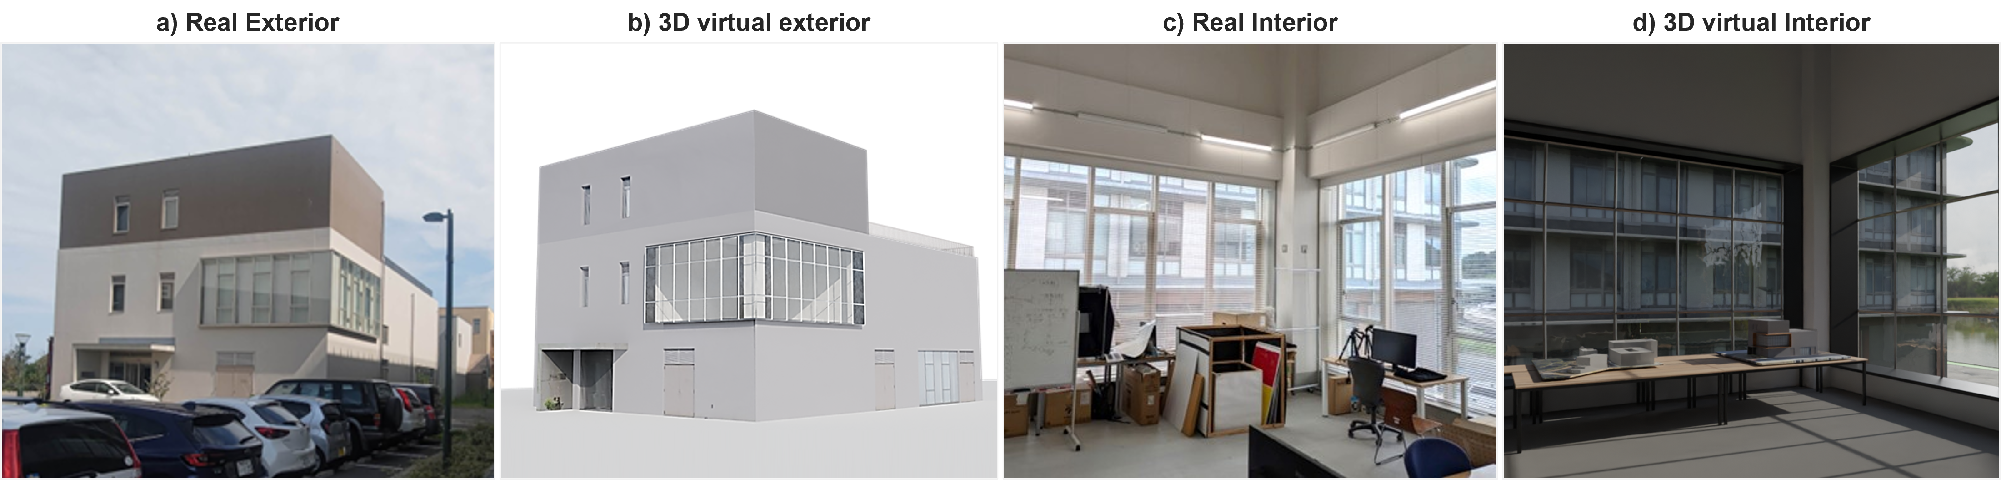
\includegraphics[width= \linewidth]{Images/Realvs3DmodelBlender}
                    \captionof{figure}{Comparison side by side of the actual Architectural Environment Building (left) with its detailed 3D virtual clone (right) created for the VR experiment for Facade complexity Analysis, demonstrating the fidelity of the digital model in replicating architectural nuances.}
                    \label{fig:RealVs3dModel}
                \end{minipage}
                \hfill % Spacing between the figures
                % Right figure
                %% FigureVR interior vs Exterior
                \begin{minipage}{0.49\textwidth}
                    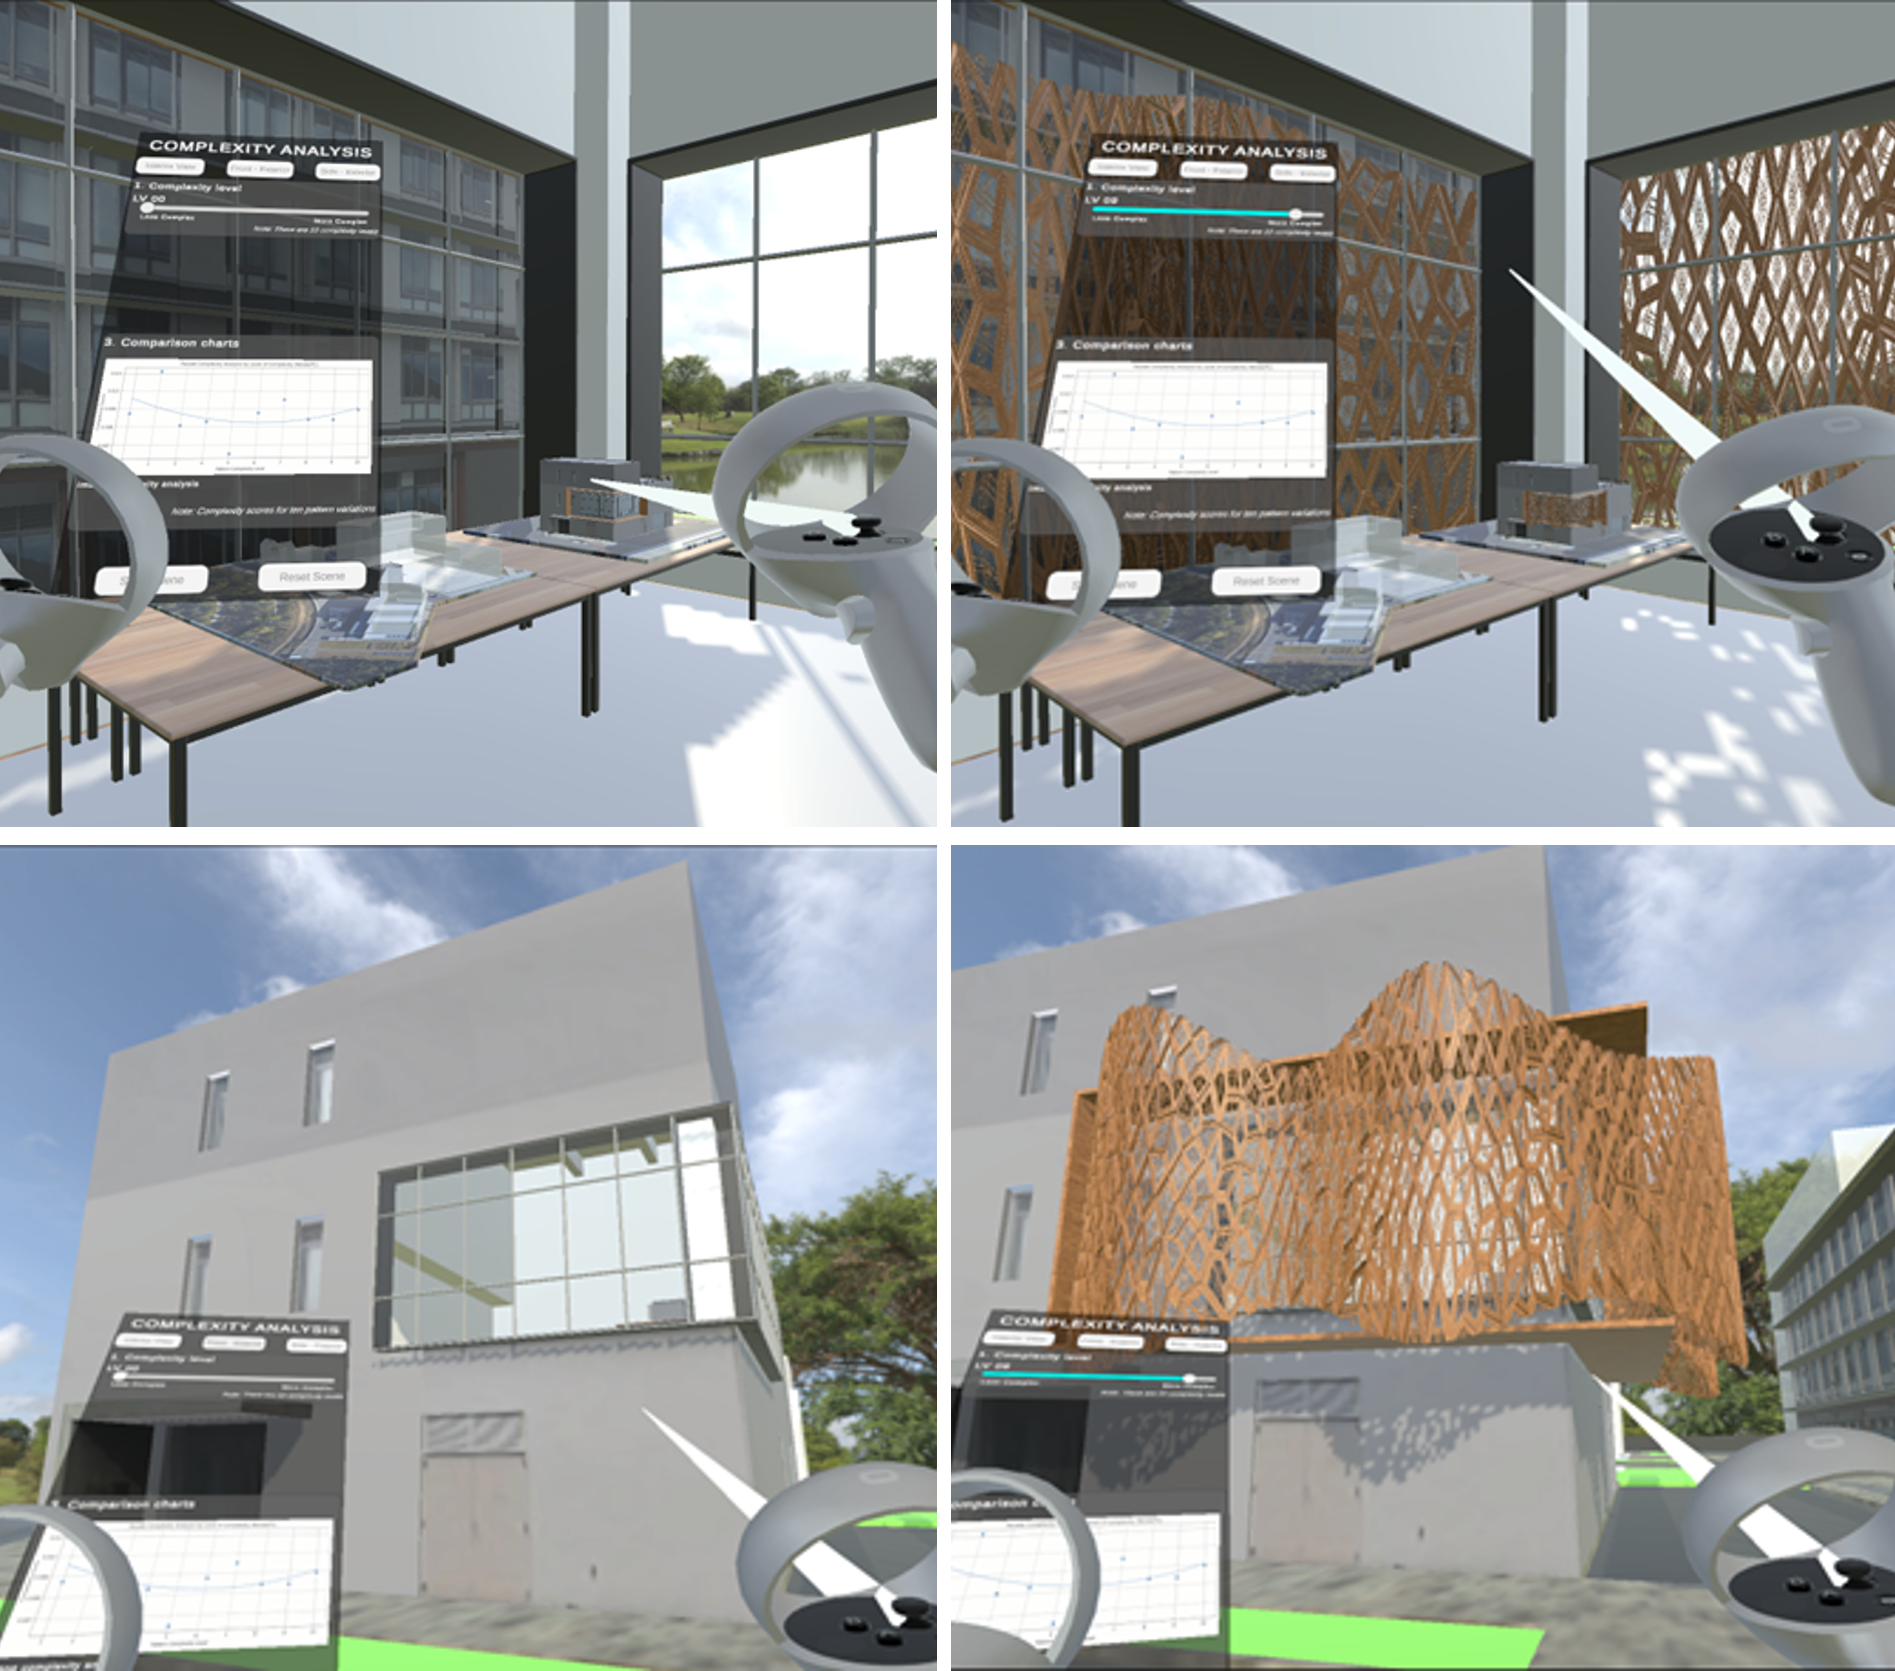
\includegraphics[width= \linewidth]{Images/VRInteriorExterior}
                    \captionof{figure}{Comparison of the VR simulation of interior (top) and exterior (bottom) of existing laboratory building as seen during the VR experiment for Facade complexity Analysis when going through the different facade variation across all three patterns.}
                    \label{fig:VRInteriorExterior}
                \end{minipage}
            \end{minipage}
        \end{tabular}
    \end{table*}

%!Figure of `Experiment Execution' flowchart
    %% Figure `Experiment Execution' flowchart
    \begin{figure*}[htb]
        \centering
        \includegraphics[width= \linewidth]{Images/FlowchartExperiment}
          \caption{`Experiment Execution' Flowchart: This flowchart outlines the three stages of the experiment, including the VR Interaction Stage (I), the Screen-Based Ranking Stage (II), and the Post-Experiment Survey (III), providing a visual representation of the sequential steps involved in the study.}
          \label{fig:ExperimentFlowchart}
    \end{figure*}

 %% CICA Flowchart
    \begin{table*}[htb]
            \centering
            \small
            \begin{tabular}{c}
                %Top cell with one figure
                %Figure Computational Image Compexity Analysis (CICA) System flowchart
                \begin{minipage}{\textwidth}
                    \centering
                    \includegraphics[width= \linewidth]{Images/CICAFlowchart}
                    \captionof{figure}{Flowchart illustrating the applications of CICA system (detailed in Section\ref{subsec:CICAsystem}), including its role in analyzing complexity scores for historical architectural styles (b) and 3D-modeled facades (a) designed with various degrees of complexity(presented in Section\ref{subsubsec:CICAfor3DmodeledFacades}).}
                    \label{fig:CICAImageEvaluationFlowchart}
                \end{minipage}
            \end{tabular}
            \end{table*}